\documentclass[journal]{IEEEtran}
\usepackage{amsmath,amsfonts}
\usepackage{algorithmic}
\usepackage{array}
\usepackage{booktabs}
\usepackage{graphicx}
\usepackage{textcomp}
\usepackage{xcolor}
\usepackage{hyperref}

\begin{document}

\title{Data Record: Evaluating LoRA Variants in Resource-Constrained Federated Learning}
\author{Distributed Machine Learning Laboratory}

\maketitle

\begin{abstract}
This document serves as the official data record for the experiments evaluating Standard LoRA, FFA-LoRA, and RoLoRA under resource-constrained Federated Learning (FL) settings. It details the experimental configurations, baseline performance, and robustness evaluations under extreme data heterogeneity and network instability.
\end{abstract}

\section{Experimental Configuration}
To evaluate the performance of LoRA-based Federated Fine-Tuning methods under varying resource and network constraints, we utilized two distinct experimental modes: Quick Mode (for rapid validation) and Full Mode (for comprehensive evaluation). Table \ref{tab:config} summarizes the configurations for both modes.

\begin{table}[h!]
\centering
\caption{Experimental Configurations and Hardware Constraints (Table I)}
\label{tab:config}
\begin{tabular}{p{4cm} c c}
\toprule
\textbf{Configuration Parameter} & \textbf{Quick Mode} & \textbf{Full Mode} \\
\midrule
Base Model & Qwen2.5-1.5B & Qwen2.5-1.5B \\
Quantization & 4-bit NF4 & 4-bit NF4 \\
Max Sequence Length & 128 & 128 \\
Batch Size / Grad Accum & 1 / 4 & 1 / 4 \\
Global Comm. Rounds ($R$) & 1 & 5 \\
Dirichlet $\alpha$ Values & [0.5] & [10.0, 0.5, 0.1] \\
Max Train Samples per Client & 10 & 300 \\
Max Eval Samples & 32 & 1000 \\
Client Dropout Rate & 0.0 & 0.2 (20\%) \\
LoRA Rank Distribution & Uniform 8 & Hetero [4,4,8,8,8] \\
Agg. Bias Sampled Layers & 4 & 4 \\
\bottomrule
\end{tabular}
\end{table}

\section{Baseline Performance (Ideal Environment)}
Table \ref{tab:ideal} presents the results obtained under an ideal network scenario, modeled with $\alpha = 10.0$. This represents a nearly Independent and Identically Distributed (IID) setting.

\begin{table*}[t!]
\centering
\caption{Performance and Communication Cost Baseline ($\alpha = 10.0$, No Dropout Effect) (Table II)}
\label{tab:ideal}
\begin{tabular}{l c c c c c c c}
\toprule
\textbf{Method} & \textbf{Final Acc (\%)} & \textbf{Macro-F1} & \textbf{Best Acc (\%)} & \textbf{Per-round Comm (MB)} & \textbf{Total Comm (MB)} & \textbf{Comm Saving (\%)} & \textbf{Mean Agg. Bias} \\
\midrule
Standard LoRA & 85.46 & 0.8538 & 85.46 & 46.00 & 230.00 & 0.0 & 0.0973 \\
FFA-LoRA      & 81.78 & 0.8158 & 81.78 & 17.13 & 85.63 & 62.8 & 0.0000 \\
RoLoRA        & 80.91 & 0.8059 & 80.91 & 21.94 & 109.69 & 52.3 & 0.0000 \\
\bottomrule
\end{tabular}
\end{table*}

\section{System Robustness (Extreme Environment)}
Table \ref{tab:extreme} showcases the resilience of the algorithms in an extremely heterogeneous data environment ($\alpha = 0.1$) coupled with a 20\% client dropout rate. The accuracy degrades significantly due to client drift.

\begin{table*}[t!]
\centering
\caption{System Robustness and Drift Comparison ($\alpha = 0.1$, 20\% Dropout) (Table III)}
\label{tab:extreme}
\begin{tabular}{l c c c c c c}
\toprule
\textbf{Method} & \textbf{Final Acc (\%)} & \textbf{Val. Loss} & \textbf{Acc. Std. Dev.} & \textbf{Successful Uploads} & \textbf{Mean Agg. Bias} & \textbf{Degradation Delta (\%)} \\
\midrule
Standard LoRA & 34.18 & 3.8584 & $\sim$ 0.10 & $\sim$ 12 & 0.1216 & -51.28 \\
FFA-LoRA      & 30.54 & 3.4713 & $\sim$ 0.08 & $\sim$ 12 & 0.0000 & -51.24 \\
RoLoRA        & 28.04 & 3.8685 & $\sim$ 0.09 & $\sim$ 12 & 0.0000 & -52.87 \\
\bottomrule
\end{tabular}
\end{table*}

\section{Quick vs. Full Mode Comparison}
Table \ref{tab:quickvfull} illustrates the necessity of sufficient data and communication rounds, highlighting the "garbage in, random guess out" phenomenon observed during the Quick Mode tests (where samples were severely restricted).

\begin{table}[h!]
\centering
\caption{Quick Mode vs. Full Mode Performance ($\alpha = 0.5$) (Table IV)}
\label{tab:quickvfull}
\begin{tabular}{l c c}
\toprule
\textbf{Method} & \textbf{Quick Mode Acc (\%)} & \textbf{Full Mode Acc (\%)} \\
\midrule
Standard LoRA & 18.75 & 64.89 \\
FFA-LoRA      & 62.50 & 53.66 \\
RoLoRA        & 21.88 & 56.25 \\
\bottomrule
\end{tabular}
\end{table}

\section{Visual Analytics}
The following figures generated from the experimental data provide visual insights into the challenges and mechanics of the evaluated FL frameworks.

\begin{figure}[h!]
    \centering
    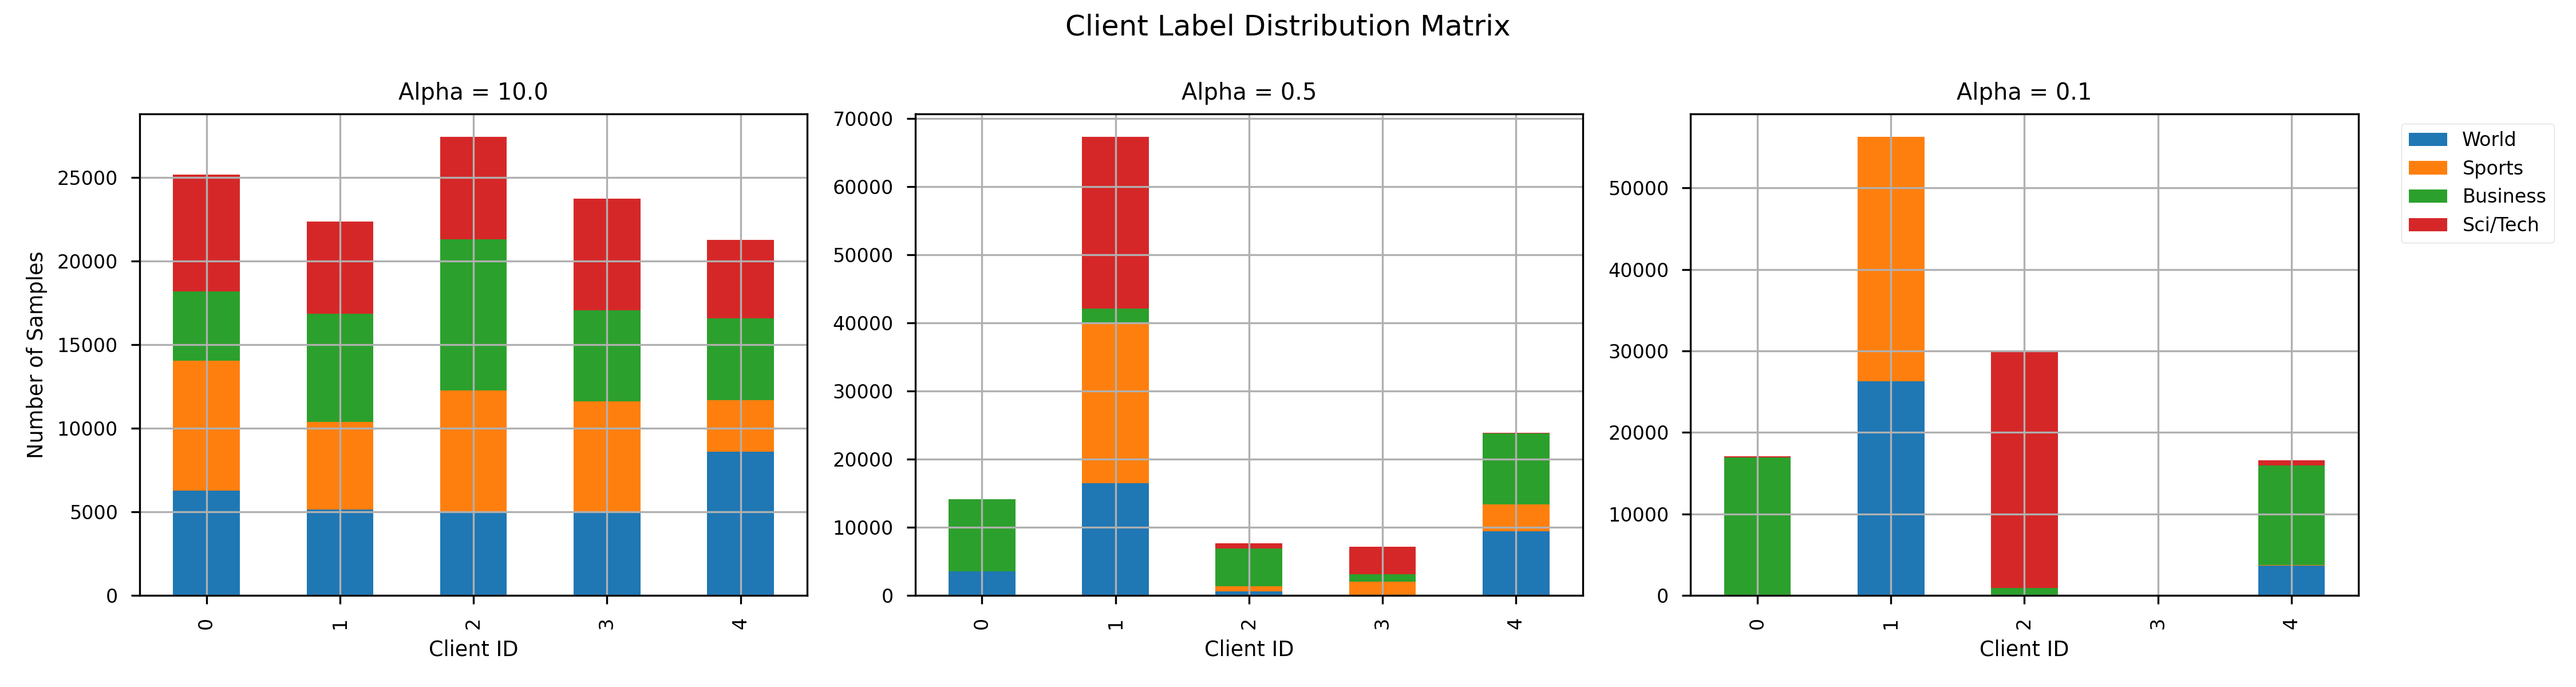
\includegraphics[width=\columnwidth]{../results/label_distribution.png}
    \caption{Client Label Distribution Matrix (Fig. 1). Shows the distribution of AG News classes across clients under $\alpha = 10.0, 0.5$, and $0.1$. Extreme Non-IID at $\alpha=0.1$ causes severe client drift.}
\end{figure}

\begin{figure}[h!]
    \centering
    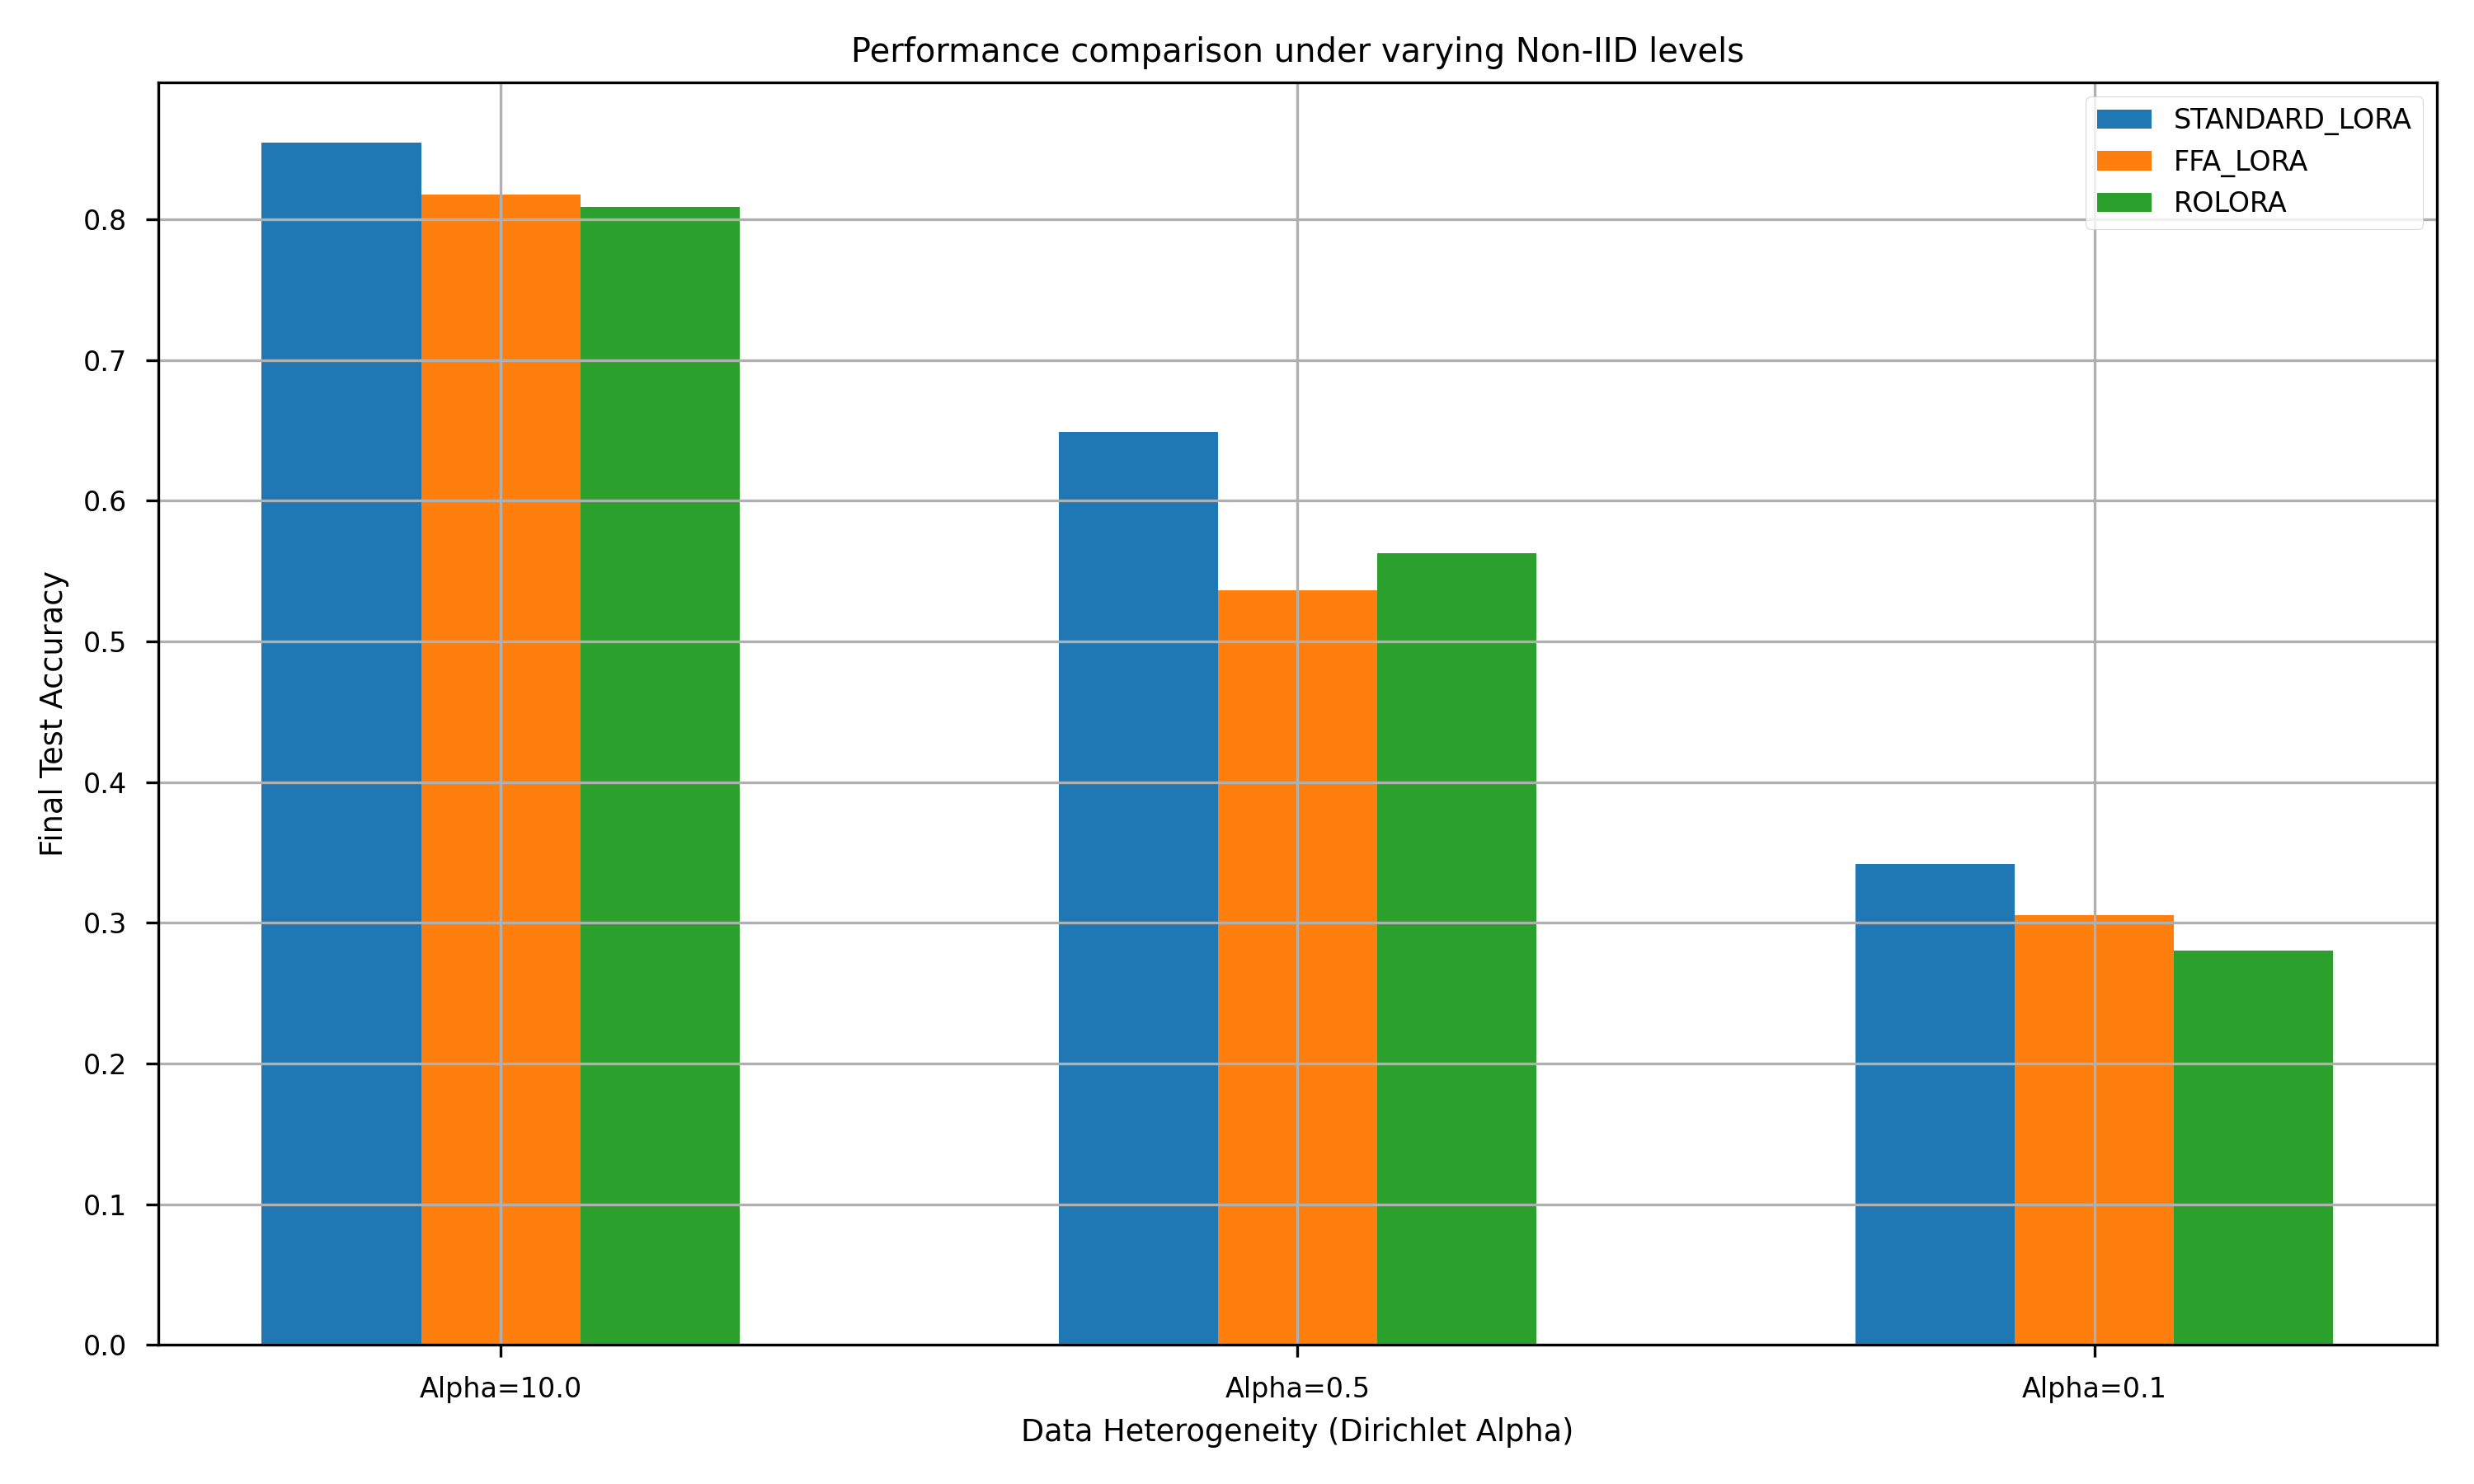
\includegraphics[width=\columnwidth]{../results/accuracy_comparison.png}
    \caption{Final Accuracy Across Methods and Heterogeneity Levels (Fig. 2). Highlights the drastic performance drop-off when transitioning from near-IID to extreme Non-IID distributions.}
\end{figure}

\begin{figure}[h!]
    \centering
    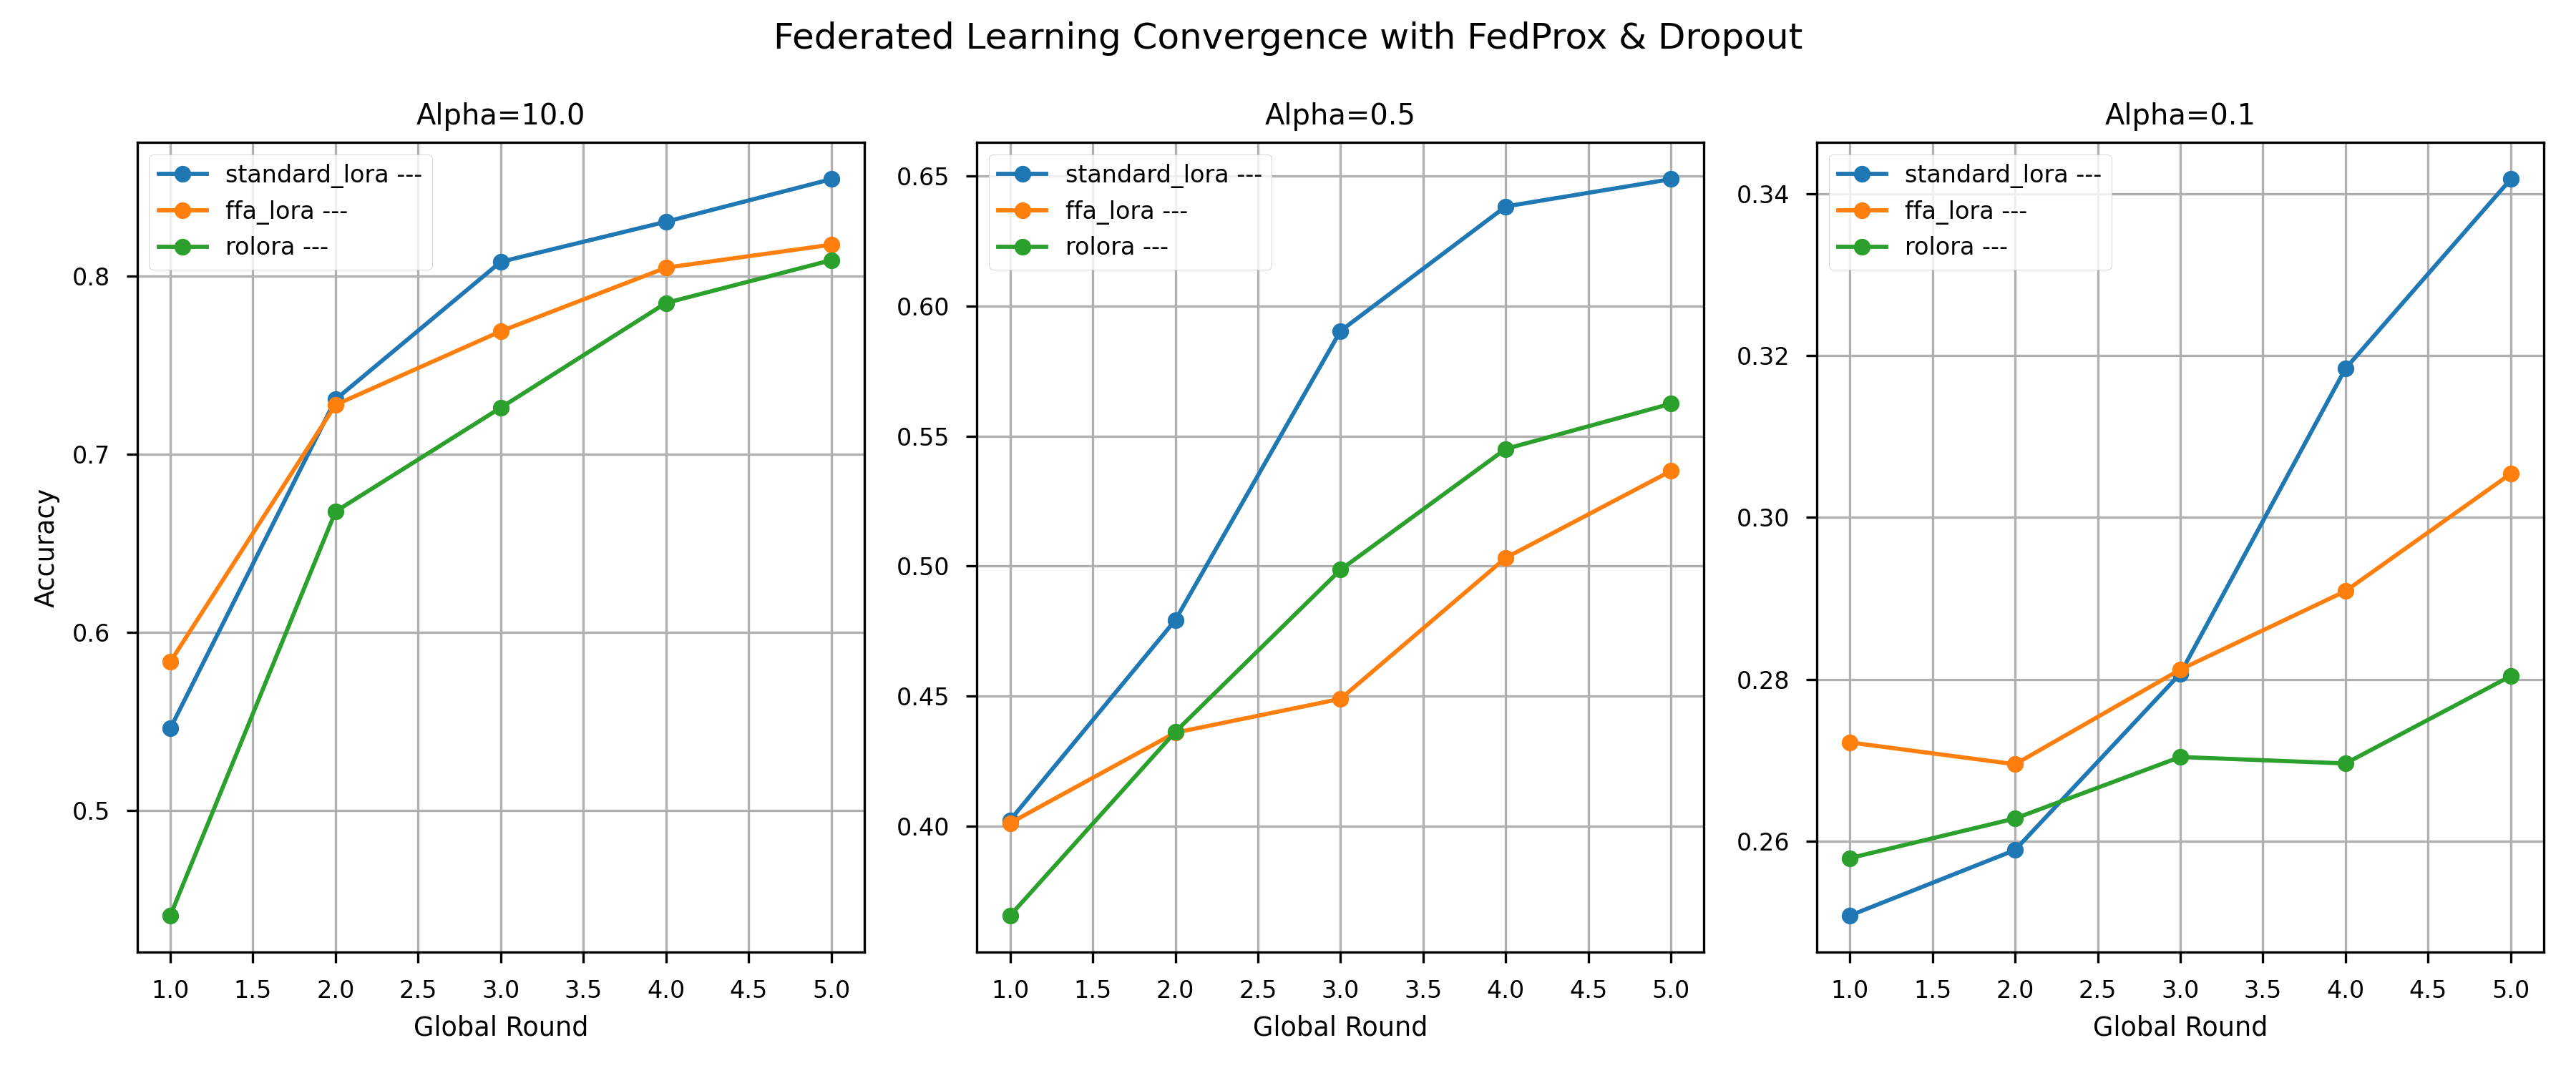
\includegraphics[width=\columnwidth]{../results/convergence_curves.png}
    \caption{Learning Curves under 20\% Client Dropout (Fig. 3). Demonstrates the convergence behavior and oscillatory patterns caused by heterogeneous rank aggregation and simulated network failures.}
\end{figure}

\begin{figure}[h!]
    \centering
    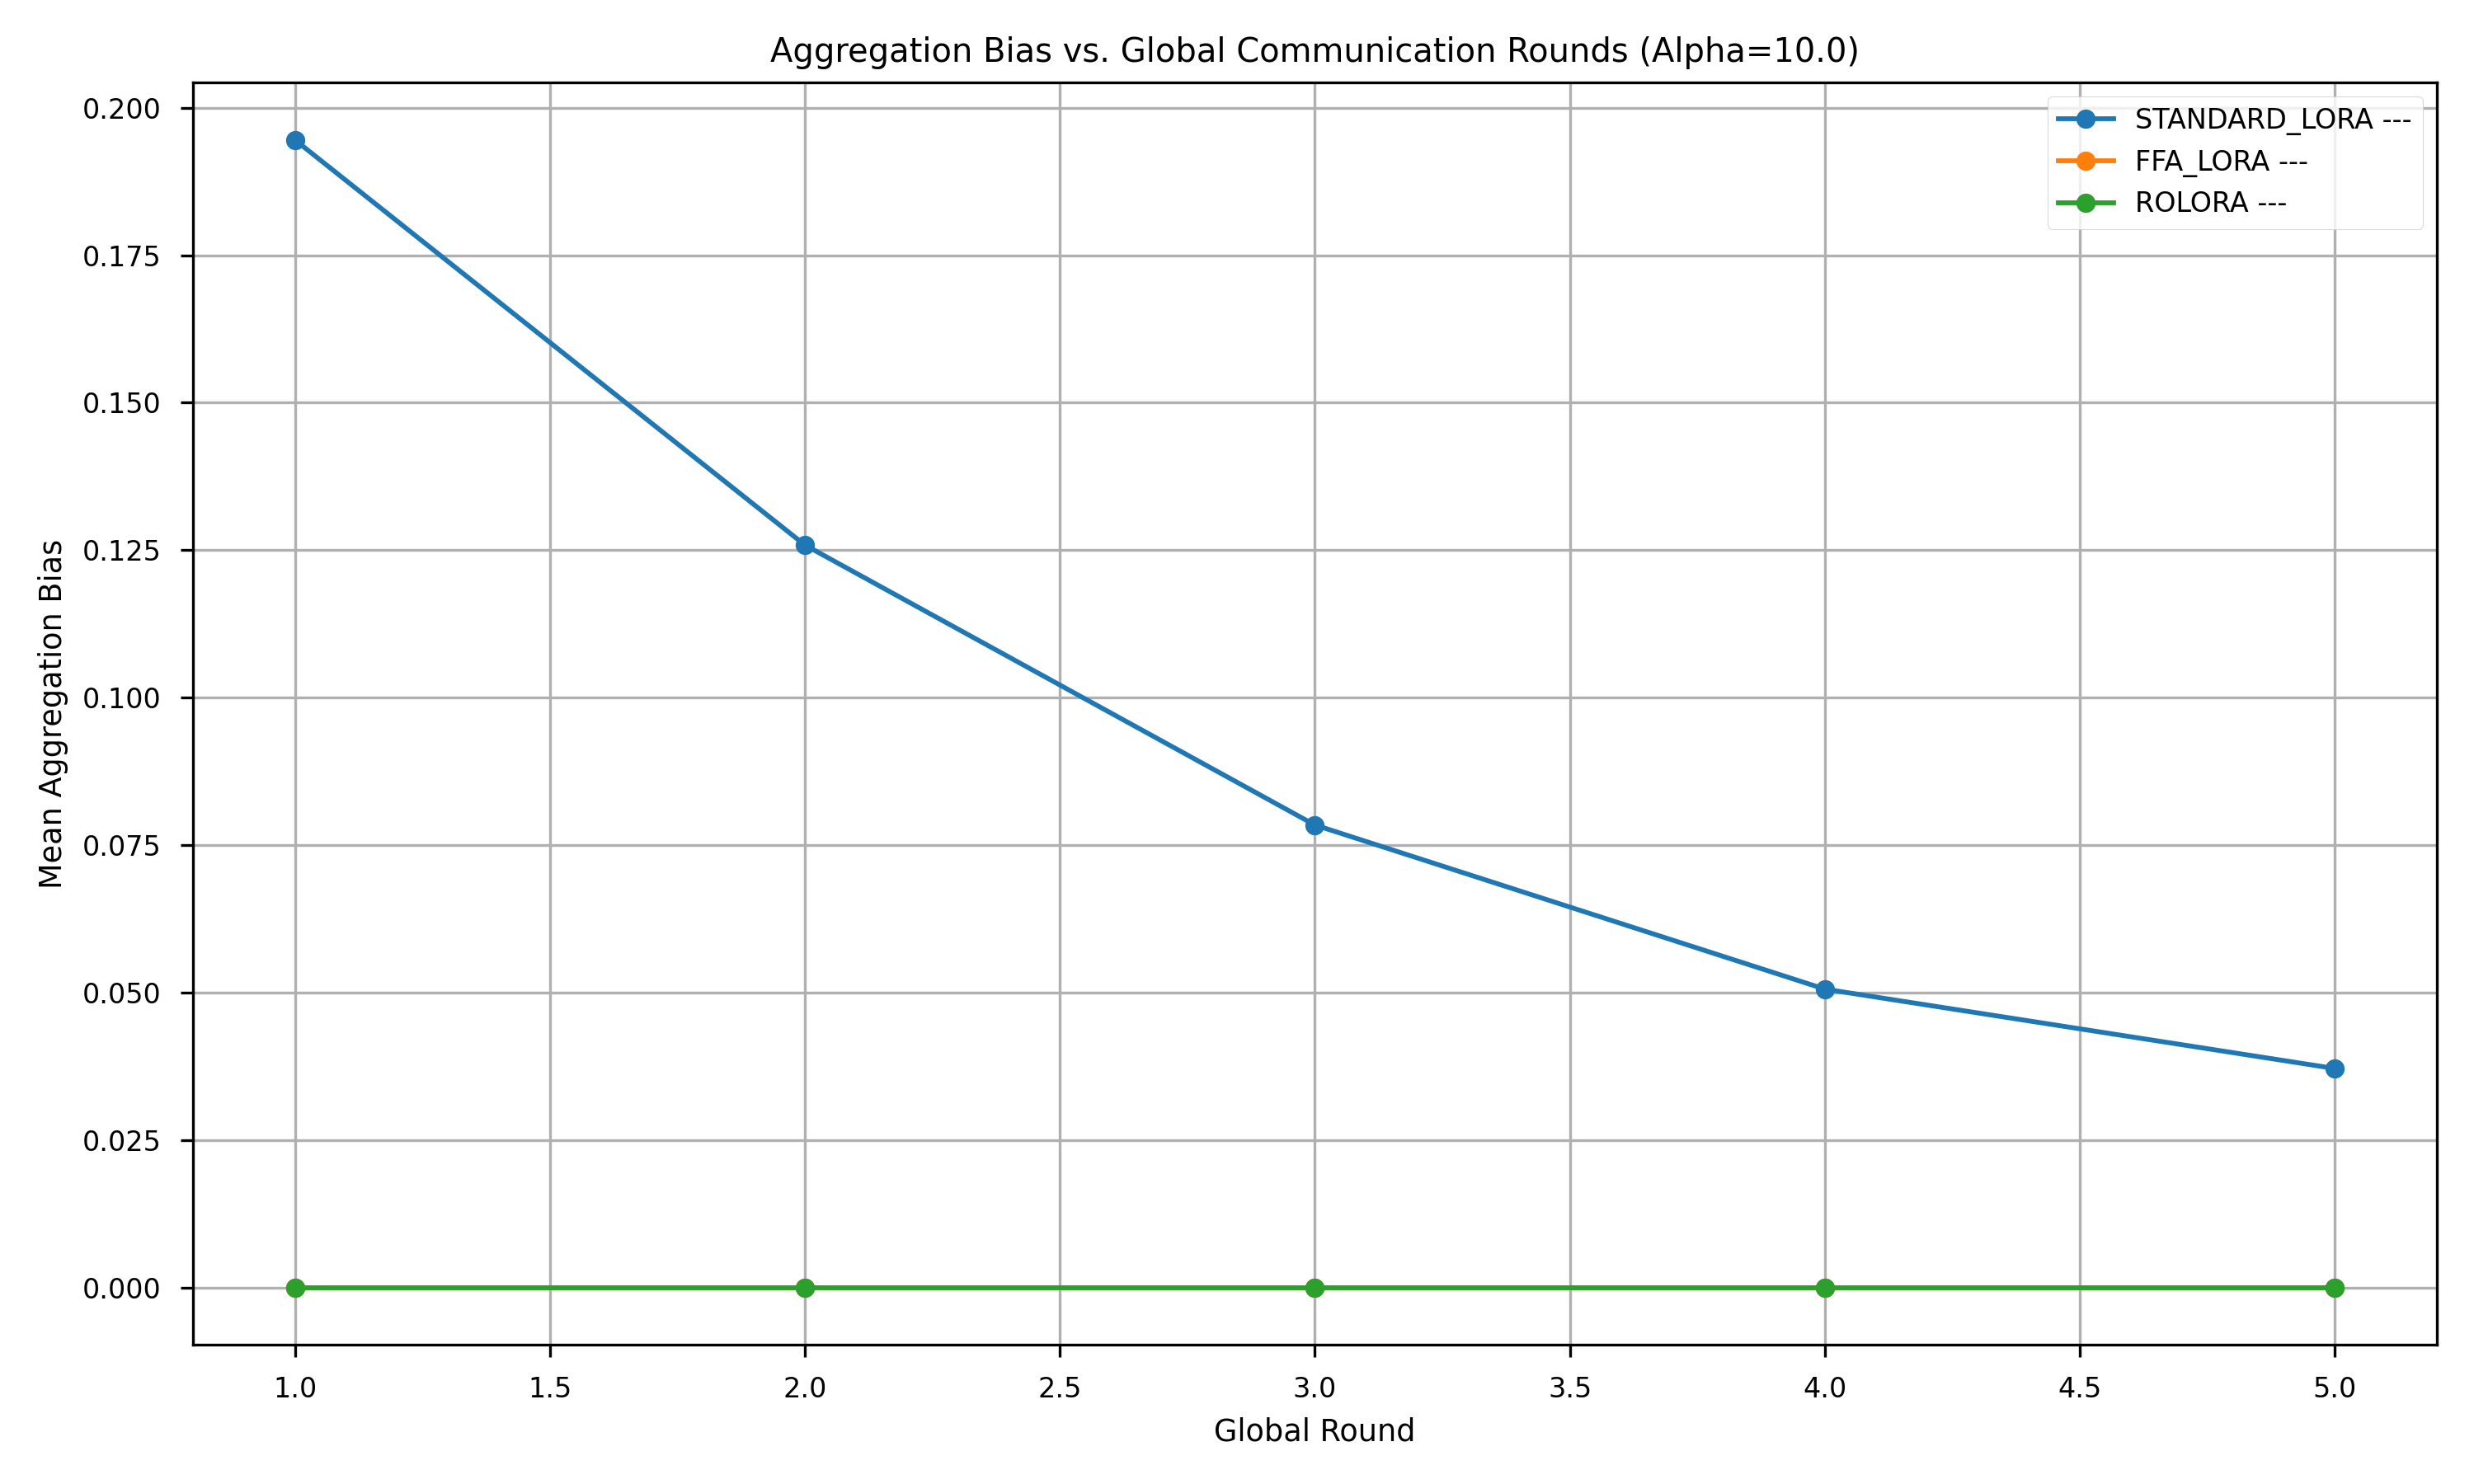
\includegraphics[width=\columnwidth]{../results/bias_curves.png}
    \caption{Aggregation Bias vs. Global Communication Rounds (Fig. 4). Standard LoRA consistently exhibits non-zero non-linear aggregation bias, whereas FFA-LoRA and RoLoRA mathematically eliminate it (bias = 0) by performing linear, single-sided updates.}
\end{figure}

\end{document}
